\documentclass[a4paper,10pt]{exam}
\usepackage[document]{ragged2e}
 \usepackage[table]{xcolor}
\usepackage{circuitikz}
\pagestyle{empty}
\usepackage{tikz}
\usepackage{multirow}
\usepackage{float}
\usepackage{amsmath}
\usepackage{multicol}
\usepackage{array}
\usepackage{enumitem}
\usepackage{setspace}
\usepackage{amssymb}


\usepackage{cite}
\usepackage{graphicx}
\usepackage{amsmath,amssymb,amsfonts,amsthm}
\usepackage{algorithmic}
\usepackage{graphicx}
\usepackage{textcomp}
\usepackage{xcolor}
\usepackage{txfonts}
\usepackage{listings}
\usepackage{enumitem}
\usepackage{mathtools}
\usepackage{gensymb}
\usepackage{comment}
\usepackage[breaklinks=true]{hyperref}
\usepackage{tkz-euclide} 
\usepackage{listings}
\usepackage{gvv}                                        
%\def\inputGnumericTable{}                                 
\usetikzlibrary{arrows.meta, positioning}
\usepackage{xparse}
\usepackage{color}                                            
\usepackage{array}                                            
\usepackage{longtable}                                       
\usepackage{calc}                                             
\usepackage{multirow}
\usepackage{multicol}
\usepackage{hhline}                                           
\usepackage{ifthen}                                           
\usepackage{lscape}
\usepackage{tabularx}
\usepackage{array}
\usepackage{float}
\newtheorem{theorem}{Theorem}[section]
\newtheorem{problem}{Problem}
\newtheorem{proposition}{Proposition}[section]
\newtheorem{lemma}{Lemma}[section]
\newtheorem{corollary}[theorem]{Corollary}
\newtheorem{example}{Example}[section]
\newtheorem{definition}[problem]{Definition}
\newcommand{\BEQA}{\begin{eqnarray}}
\newcommand{\EEQA}{\end{eqnarray}}
\usepackage{float}
%\newcommand{\define}{\stackrel{\triangle}{=}}
\theoremstyle{remark}
\usepackage{circuitikz}
\usepackage{tikz}
\usepackage{ragged2e}

\begin{document}
\raggedright{\textbf{GATE 2019 General Aptitude (GA) Set-3}}\\
\hrule
\vspace{1cm}
\textbf{Q.1-Q.5 carry one mark each.}
\begin{enumerate}
\item I am not sure if the bus that has been booked will be able to \rule{2cm}{0.15mm} all the students.\hfill{(GATE EE 2019)}
\begin{multicols}{4}
\begin{enumerate}
\item sit
\item deteriorate
\item fill
\item accommodate
\end{enumerate}
\end{multicols}
\item  The passengers were angry \rule{2cm}{0.15mm} the airline staff about the delay.\hfill{(GATE EE 2019)}
\begin{multicols}{4}
\begin{enumerate}
\item on
\item about
\item with
\item towards
\end{enumerate}
\end{multicols}
\item The missing number in the given sequence 343, 1331,\rule{1cm}{0.15mm}, 4913 is\hfill{(GATE EE 2019)}
\begin{multicols}{4}
\begin{enumerate}
\item 3375
\item 2744
\item 2197
\item 4096
\end{enumerate}
\end{multicols}
\item It takes two hours for a person X to mow the lawn. Y can mow the same lawn in four hours. How long (in minutes) will it take X and Y, if they work together to mow the lawn?\hfill{(GATE EE 2019)}
\begin{multicols}{4}
\begin{enumerate}
\item 60
\item 80
\item 90
\item 120
\end{enumerate}
\end{multicols}
\item  Newspapers are a constant source of delight and recreation for me. The \rule{1cm}{0.15mm} trouble is that I read  \rule{1cm}{0.15mm}many of them.\hfill{(GATE EE 2019)}
\begin{multicols}{4}
\begin{enumerate}
\item even, quite
\item even, too
\item only, quite
\item only, too
\end{enumerate}
\end{multicols}
\textbf{Q.6-Q.10 carry two marks each.}
\item How many integers are there between 100 and 1000 all of whose digits are even?\hfill{(GATE EE 2019)}
\begin{multicols}{4}
\begin{enumerate}
\item 60
\item 80
\item 100
\item 90
\end{enumerate}
\end{multicols}
\item The ratio of the number of boys and girls who participated in an examination is 4:3. The total percentage of candidates who passed the examination is 80 and the percentage of girls who passed is 90. The percentage of boys who passed is
 \rule{1.5cm}{0.15mm}.\hfill{(GATE EE 2019)}
\begin{multicols}{4}
\begin{enumerate}
\item 55.50
\item 72.50
\item 80.50
\item 90.00
\end{enumerate}
\end{multicols}
\vfill
\noindent\rule{\linewidth}{0.4pt}
GA \hfill 1/2
\newpage
\raggedright{\textbf{GATE 2019 General Aptitude (GA) Set-3}}\\
\vspace{2.5mm}
\noindent\rule{\linewidth}{0.4pt}
\item An award-winning study by a group of researchers suggests that men are as prone to buying on impulse as women but women feel more guilty about shopping.\\
Which one of the following statements can be inferred from the given text?\hfill{(GATE EE 2019)}
\begin{enumerate}
    \item Some men and women indulge in buying on impulse
    \item All men and women indulge in buying on impulse
    \item Few men and women indulge in buying on impulse
    \item Many men and women indulge in buying on impulse
\end{enumerate}
\item  Given two sets $ X = \{ 1, 2, 3 \}$  and $ Y = \{ 2, 3, 4 \} $, we construct a set Z of all possible fractions where the numerators belong to set X and the denominators belong to set Y.The product of elements having minimum and maximum values in the set Z is \rule{1.5cm}{0.15mm} .\hfill{(GATE EE 2019)}
\begin{multicols}{4}
\begin{enumerate}
\item $\frac{1}{12}$
\item $\frac{1}{8}$
\item $\frac{1}{6}$
\item $\frac{3}{8}$
\end{enumerate}
\end{multicols}

\item Consider five people -- Mita, Ganga, Rekha, Lakshmi and Sana. Ganga is taller than both Rekha and Lakshmi. Lakshmi is taller than Sana. Mita is taller than Ganga. Which of the following conclusions are true?\hfill{(GATE EE 2019)}
\begin{enumerate}
    \item Lakshmi is taller than Rekha
    \item Rekha is shorter than Mita
    \item Rekha is taller than Sana
    \item Sana is shorter than Ganga
\end{enumerate}

\begin{enumerate}
\item 1 and 3
\item 3 only
\item 2 and 4
\item 1 only
\end{enumerate}

\vspace{1cm}

\begin{center}
    \textbf{END OF THE QUESTION PAPER}
\end{center}
\vfill
\noindent\rule{\linewidth}{0.4pt}
GA \hfill 2/2
\newpage
\raggedright{GATE 2019 Electrical Engineering (Set No)}

\noindent\rule{\linewidth}{0.4pt}
\textbf{Q.1 - Q.25 carry ONE mark each.}
\begin{enumerate}[label=\arabic*.]
\item The inverse Laplace transform of H(s)= $\frac{s+3}{s^{2}+2s+1}$ for t $\geq
$ 0 is\hfill{(GATE EE 2019)}
\begin{multicols}{2}
\begin{enumerate}
\item $3t e^{-t} + e^{-t}$ 
\item $3e^{-t}$ 
\item $2t e^{-t} + e^{-t}$ 
\item $4te^{-t} + e^{-t}$
\end{enumerate}
\end{multicols}
\item M is 2x2 matrix with eigenvalues 4 and 9.The eigenvalues of $M^{2}$ are\hfill{(GATE EE 2019)}
\begin{multicols}{4}
\begin{enumerate}
\item 4 and 9
\item 2 and 3
\item -2 and -3
\item 16 and 81
\end{enumerate}
\end{multicols}
\item The partial differential equation\\
$\frac{\partial^2 u}{\partial t^2} - c^2 \left( \frac{\partial^2 u}{\partial x^2} + \frac{\partial^2 u}{\partial y^2} \right) = 0 ;\quad \text{where } c \neq 0$ \\
is known as\hfill{(GATE EE 2019)}
\begin{multicols}{2}
\begin{enumerate}
\item heat equation 
\item wave equation
\item Poisson's equation
\item Laplace equation
\end{enumerate}
\end{multicols}
\item Which one of the following functions is analytic in the region $|z| $ $\leq$ 1?\hfill{(GATE EE 2019)}
\begin{multicols}{4}
\begin{enumerate}
\item $\frac{z^{2}-1}{z}$
\item $\frac{z^{2}-1}{z+2}$
\item $\frac{z^{2}-1}{z-0.5}$
\item $\frac{z^{2}-1}{z+j0.5}$
\end{enumerate}
\end{multicols}
\item The mean-square of a zero-mean random process is $ \frac{kT}{C} $, where k is Boltzmann's constant,T is the absolute temperature, and C is a capacitance. The standard deviation of the random process is\hfill{(GATE EE 2019)}
\begin{multicols}{4}
\begin{enumerate}
\item $\frac{kT}{C}$
\item $\sqrt{\frac{kT}{C}}$
\item $\frac{C}{kT}$
\item $\frac{\sqrt{kT}}{C}$
\end{enumerate}
\end{multicols}
\item 
A system transfer function is $$ H(s) = \frac{a_1 s^2 + b_1 s + c_1}{a_2 s^2 + b_2 s + c_2} $$. If $ a_1 = b_1 = 0 $, and all other coefficients are positive, the transfer function represents a\hfill{(GATE EE 2019)}
\begin{enumerate}
\item low pass filter
\item high pass filter
\item band pass filter
\item notch filter
\end{enumerate}
\item The symbols,  a and T, represent positive quantities, and $u(t)$ is the unit step function. Which one of the following impulse responses is NOT the output of a causal linear time-invariant system?\hfill{(GATE EE 2019)}
\begin{multicols}{2}
\begin{enumerate}
\item $e^{a t}u(t)$
\item $e^{-a(t+T)}u(t)$
\item $1 + e^{-a t}u(t)$
\item $e^{-a(t-T)}u(t)$
\end{enumerate}
\end{multicols}
\item A 5 kVA, 50 V/100 V, single-phase transformer has a secondary terminal voltage of 95 V when loaded. The regulation of the transformer is\hfill{(GATE EE 2019)}
\begin{multicols}{4}
\begin{enumerate}
\item 4.5\%
\item 9\%
\item 5\%
\item 1\%
\end{enumerate}
\end{multicols}
\vfill
\noindent\rule{\linewidth}{0.4pt}
EE \hfill 1/13
\newpage
\raggedright{GATE 2019 Electrical Engineering (Set No)}
\noindent\rule{\linewidth}{0.4pt}

\item A six-pulse thyristor bridge rectifier is connected to a balanced three-phase, 50 Hz AC source. Assuming that the DC output current of the rectifier is constant, the lowest harmonic component in the AC input current is\hfill{(GATE EE 2019)}
\begin{multicols}{4}
\begin{enumerate}
    \item 100 Hz
    \item 150 Hz
    \item 250 Hz
    \item 300 Hz
\end{enumerate}
\end{multicols}

\item The parameter of an equivalent circuit of a three-phase induction motor affected by reducing the rms value of the supply voltage at the rated frequency is\hfill{(GATE EE 2019)}
\begin{enumerate}
    \item rotor resistance
    \item rotor leakage reactance
    \item magnetizing reactance
    \item stator resistance
\end{enumerate}
\item A three-phase synchronous motor draws 200 A from the line at unity power factor at rated load. Considering the same line voltage and load, the line current at a power factor of 0.5 leading is\hfill{(GATE EE 2019)}
\begin{multicols}{4}
\begin{enumerate}
    \item 100 A
    \item 200 A
    \item 300 A
    \item 400 A
\end{enumerate}
\end{multicols}

\item In the circuit shown below, the switch is closed at $t = 0$ . The value of $\theta$ in degrees which will give the maximum value of DC offset of the current at the time of switching is\hfill{(GATE EE 2019)}
\begin{figure}[H]
    \centering
    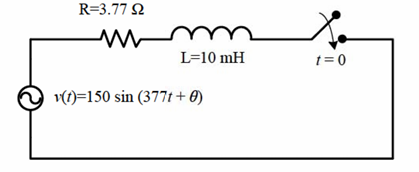
\includegraphics[width=0.6\columnwidth]{figs/Q 12.png}\caption{}     \label{fig:placeholder}
\end{figure}
\begin{multicols}{4}
\begin{enumerate}
    \item 60
    \item $-45$
    \item 90
    \item $-30$
\end{enumerate}
\end{multicols}

\item The output response of a system is denoted as $y(t)$, and its Laplace transform is given by
$Y(s) = \frac{10}{s(s^2 + s + 100\sqrt{2})}$
The steady state value of $ y(t) $is\hfill{(GATE EE 2019)}
\begin{multicols}{4}
\begin{enumerate}
    \item $\frac{1}{10\sqrt{2}}$ 
    \item $10\sqrt{2}$ 
    \item $\frac{1}{100\sqrt{2}}$ 
    \item $100\sqrt{2}$
\end{enumerate}
\end{multicols}

\item The open loop transfer function of a unity feedback system is given by
$G(s) = \frac{\pi e^{-0.25s}}{s}$
In G(s) plane, the Nyquist plot of G(s) passes through the negative real axis at the point\hfill{(GATE EE 2019)}
\begin{multicols}{4}
\begin{enumerate}
    \item $(-0.5, j0)$
    \item $(-0.75, j0)$ 
    \item $(-1.25, j0)$
    \item $(-1.5, j0)$
\end{enumerate}
\end{multicols}

\item The characteristic equation of a linear time-invariant (LTI) system is given by
$\Delta(s) = s^4 + 3s^3 + 3s^2 + s + k = 0.
$
The system is BIBO stable if\hfill{(GATE EE 2019)}
\begin{multicols}{4}
\begin{enumerate}
    \item $0 < k < \frac{12}{9}$
    \item $k > 3$
    \item $0 < k < \frac{8}{9}$
    \item $k > 6$
\end{enumerate}
\end{multicols}
\vfill
\noindent\rule{\linewidth}{0.4pt}
EE \hfill 2/13
\newpage
\raggedright{GATE 2019 Electrical Engineering (Set No)}
\noindent\rule{\linewidth}{0.4pt}

\item Given, $ V_{gs}$ is the gate-source voltage, $V_{ds}$ is the drain source voltage, and $V_{th}$ is the threshold voltage of an enhancement type NMOS transistor, the conditions for transistor to be biased in saturation are\hfill{(GATE EE 2019)}
\begin{enumerate}
    \item $ V_{gs} < V_{th} ;\  V_{ds} \geq V_{gs} - V_{th} $
    \item $ V_{gs} >  V_{th} ;\  V_{ds} \geq V_{gs} - V_{th} $
    \item $ V_{gs} > V_{th} ;\  V_{ds} \leq V_{gs} - V_{th} $
    \item $ V_{gs} < V_{th} ;\  V_{ds} \leq V_{gs} - V_{th} $
\end{enumerate}

\item A current controlled current source (CCCS) has an input impedance of 10$\Omega$ and output impedance of 100k$\Omega$. When this CCCS is used in a negative feedback closed loop with a loop gain of 9, the closed loop output impedance is\hfill{(GATE EE 2019)}
\begin{multicols}{4}
\begin{enumerate}
    \item 10 $\Omega$
    \item 100 $\Omega$
    \item 100 k$\Omega$
    \item 1000 k$\Omega$
\end{enumerate}
\end{multicols}

\item If $f = 2x^3 + 3y^2 + 4z $, the value of line integral $\int_C \nabla f \cdot d\mathbf{r}$ evaluated over contour $C$ formed by the segments $(-3, -3, 2) \to (2, -3, 2) \to (2, 6, 2) \to (2, 6, -1)$ is \rule{2cm}{0.15mm}.\hfill{(GATE EE 2019)}

\item The current $I$ flowing in the circuit shown below in amperes (round off to one decimal place) is  \rule{2cm}{0.15mm}.\hfill{(GATE EE 2019)}
\begin{figure}[H]
    \centering
    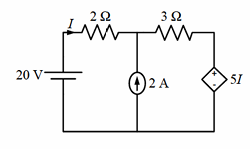
\includegraphics[width=0.5\columnwidth]{figs/Q 19.png}\caption{}     \label{fig:placeholder}
\end{figure}

\item A co-axial cylindrical capacitor shown in Figure (i) has dielectric with relative permittivity $\varepsilon_{r1} = 2$. When one-fourth portion of the dielectric is replaced with another dielectric of relative permittivity $\varepsilon_{r2}$, as shown in Figure (ii), the capacitance is doubled. The value of $\varepsilon_{r2}$ is\hfill{(GATE EE 2019)}
\begin{figure}[H]
    \centering
    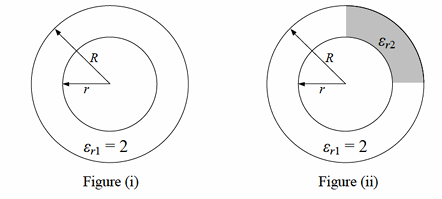
\includegraphics[width=0.75\columnwidth]{figs/Q 20.png}\caption{}     \label{fig:placeholder}
\end{figure}
\vfill
\noindent\rule{\linewidth}{0.4pt}
EE \hfill 3/13
\newpage
\raggedright{GATE 2019 Electrical Engineering (Set No)}
\noindent\rule{\linewidth}{0.4pt}
\item The $Y_{bus}$ matrix of a two-bus power system having two identical parallel lines connected between them in pu is given as
$
Y_{bus} =  \begin{bmatrix}
-j8 & j20 \\
j20 & -j8
\end{bmatrix}
$\\
The magnitude of the series reactance of each line in pu (round off up to one decimal place) is \rule{2cm}{0.15mm} .\hfill{(GATE EE 2019)}
\vspace{0.4cm}

\item Five alternators each rated 5 MVA, 13.2 kV with 25\% of reactance on its own base are connected in parallel to a busbar. The short-circuit level in MVA at the busbar is \rule{2cm}{0.15mm}.\hfill{(GATE EE 2019)}
\vspace{1cm}
\item The total impedance of the secondary winding, leads, and burden of a 5 A CT is 0.01 $\Omega$. If the fault current is 20 times the rated primary current of the CT, the VA output of the CT is \rule{2cm}{0.15mm}.\hfill{(GATE EE 2019)}
\vspace{0.3cm}
\item The rank of the matrix, $M =  \begin{bmatrix}
0 & 1 & 1\\
1 & 0 & 1\\
1 & 1 & 0
\end{bmatrix}$, is \rule{2cm}{0.15mm}.\hfill{(GATE EE 2019)}
\vspace{0.4cm}

\item The output voltage of a single-phase full bridge voltage source inverter is controlled by unipolar PWM with one pulse per half cycle. For the fundamental rms component of output voltage to be 75\% of DC voltage, the required pulse width in degrees (round off up to one decimal place) is \rule{2cm}{0.15mm}.\hfill{(GATE EE 2019)}
\vfill
\noindent\rule{\linewidth}{0.4pt}
EE \hfill 4/13
\newpage
\raggedright{GATE 2019 Electrical Engineering (Set No)}
\noindent\rule{\linewidth}{0.4pt}
\textbf{Q.26-Q.55 carry TWO marks each.}
\item Consider a $2 \times 2$ matrix $ M = [\mathbf{v}_1 \quad \mathbf{v}_2] $, where, $\mathbf{v}_1$ and $\mathbf{v}_2$ are the column vectors. Suppose $M^{-1} =  \begin{bmatrix} \mathbf{u}_1^T \\ \mathbf{u}_2^T \end{bmatrix}$, where $\mathbf{u}_1^T$ and $\mathbf{u}_2^T$ are the row vectors. Consider the following statements:

Statement 1: $\mathbf{u}_1^T \mathbf{v}_1 = 1$ and $\mathbf{u}_2^T \mathbf{v}_2 = 1$ \\
Statement 2: $\mathbf{u}_1^T \mathbf{v}_2 = 0$ and $\mathbf{u}_2^T \mathbf{v}_1 = 0$

Which of the following options is correct?\hfill{(GATE EE 2019)}

\begin{multicols}{2}
\begin{enumerate}
    \item Statement 1 is true and statement 2 is false
    \item Statement 2 is true and statement 1 is false
    \item Both the statements are true
    \item Both the statements are false
\end{enumerate}
\end{multicols}

\item The closed loop line integral
$
\oint_{|z|=5} \frac{z^3 + z^2 + 8}{z+2}\, dz
$
evaluated counter-clockwise, is\hfill{(GATE EE 2019)}

\begin{multicols}{4}
\begin{enumerate}
\item $+8\pi$
\item $-8\pi$
\item $-4\pi$
\item $+4\pi$
\end{enumerate}
\end{multicols}

\item A periodic function $f(t)$, with a period of $2\pi$, is represented as its Fourier series,
$
f(t) = a_0 + \sum_{n=1}^{\infty} a_n \cos nt + \sum_{n=1}^{\infty} b_n \sin nt.
$
If
$
f(t) = \begin{cases}
A \sin t, & 0 \leq t \leq \pi \\
0, & \pi < t < 2\pi
\end{cases},
$
the Fourier series coefficients $a_1$ and $b_1$ of $f(t)$ are\hfill{(GATE EE 2019)}

\begin{multicols}{2}
\begin{enumerate}
    \item $a_1 = \frac{A}{\pi};\; b_1 = 0$
    \item $a_1 = \frac{A}{2};\; b_1 = 0$
    \item $a_1 = 0;\; b_1 = \frac{A}{\pi}$
    \item $a_1 = 0;\; b_1 = \frac{A}{2}$
\end{enumerate}
\end{multicols}
\vfill
\noindent\rule{\linewidth}{0.4pt}
EE \hfill 5/13
\newpage
\raggedright{GATE 2019 Electrical Engineering (Set No)}
\noindent\rule{\linewidth}{0.4pt}
\item The asymptotic Bode magnitude plot of a minimum phase transfer function G(s) is shown below.\hfill{(GATE EE 2019)}
\begin{figure}[H]
    \centering
    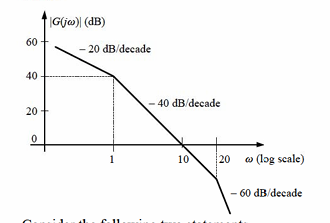
\includegraphics[width=0.5\columnwidth]{figs/Q 29.png}
    \caption{}
    \label{fig:placeholder}
\end{figure}
Consider the following two statements.\\
Statement I:Transfer function $G(s)$ has three poles and one zero.\\
Statement II:At very high frequency ($ \omega \to \infty $), the phase angle $ \angle G(j\omega) = -\frac{3\pi}{2} $.

\begin{enumerate}
\item Statement I is true and statement II is false.
\item Statement I is false and statement II is true.
\item Both the statements are true.
\item Both the statements are false.
\end{enumerate}
\item The transfer function of a phase lead compensator is given by
$
D(s) = \frac{3 \left( s + \frac{1}{3T} \right)}{s + \frac{1}{T}}.
$
The frequency (in rad/sec), at which $ \angle D(j\omega)$  is maximum, is\hfill{(GATE EE 2019)}
\begin{multicols}{4}
\begin{enumerate}
    \item $\sqrt{\frac{3}{T^2}}$
    \item $\sqrt{\frac{1}{3T^2}}$
    \item $\sqrt{3T}$
    \item $\sqrt{3T^2}$
\end{enumerate}
\end{multicols}
\item Consider a state-variable model of a system
$
 \begin{bmatrix}
\dot{x}_1 \\
\dot{x}_2
\end{bmatrix}
=
 \begin{bmatrix}
0 & 1 \\
-\alpha & -2\beta
\end{bmatrix}
 \begin{bmatrix}
x_1 \\
x_2
\end{bmatrix}
+
 \begin{bmatrix}
0 \\
\alpha
\end{bmatrix}
r
$\\
$y = [1 \;\; 0]
 \begin{bmatrix}
x_1 \\
x_2
\end{bmatrix}$
where $y$ is the output, and $r$ is the input. The damping ratio $\xi$ and the undamped natural frequency $\omega_n$ (rad/sec) of the system are given by\hfill{(GATE EE 2019)}
\begin{enumerate}
\item $\xi = \dfrac{\beta}{\sqrt{\alpha}}; \omega_n = \sqrt{\alpha}$
\item $\xi = \sqrt{\alpha}; \omega_n = \dfrac{\beta}{\sqrt{\alpha}}$
\item $\xi = \dfrac{\sqrt{\alpha}}{\beta};\omega_n = \sqrt{\beta}$
\item$\xi = \sqrt{\beta};\omega_n = \sqrt{\alpha}$
\end{enumerate}
\item A moving coil instrument having a resistance of 10$\Omega$, gives a full-scale deflection when the current is 10mA. What should be the value of the series resistance, so that it can be used as a voltmeter for measuring potential difference up to 100V?\hfill{(GATE EE 2019)}
\begin{multicols}{4}
\begin{enumerate}
    \item 9~$\Omega$
    \item 99~$\Omega$
    \item 990~$\Omega$
    \item 9990~$\Omega$
\end{enumerate}
\end{multicols}
\vfill
\noindent\rule{\linewidth}{0.4pt}
EE \hfill 6/13
\newpage
\raggedright{GATE 2019 Electrical Engineering (Set No)}
\noindent\rule{\linewidth}{0.4pt}


\item The enhancement type MOSFET in the circuit below operates according to the square law.\\
$\mu_n C_{ox} = 100~\mu A V^2$, the threshold voltage (V$_T$) is 500mV. Ignore channel length modulation. The output voltage V$_{out}$ is\hfill{(GATE EE 2019)}
\begin{figure}[H]
    \centering
    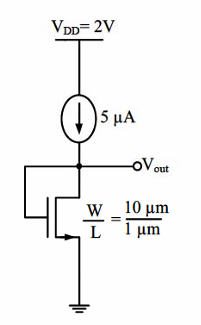
\includegraphics[width=0.3\columnwidth]{figs/Q 33.png}\caption{}     \label{fig:placeholder}
\end{figure}

\begin{multicols}{4}
\begin{enumerate}
    \item 100mV
    \item 500mV
    \item 600mV
    \item 2 V
\end{enumerate}
\end{multicols}
\item In the circuit below, the operational amplifier is ideal. If $V_1 = 10~\text{mV}$ and $V_2 = 50~\text{mV}$, the output voltage (V$_{out}$) is\hfill{(GATE EE 2019)}

\begin{figure}[H]
    \centering
    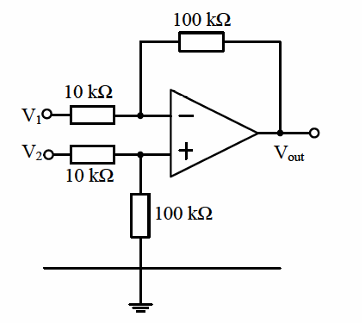
\includegraphics[width=0.4\columnwidth]{figs/Q 34.png}\caption{}     \label{fig:placeholder}
\end{figure}
\begin{multicols}{4}
\begin{enumerate}
    \item 100mV
    \item 400mV
    \item 500mV
    \item 600mV
\end{enumerate}
\end{multicols}
\vfill
\noindent\rule{\linewidth}{0.4pt}
EE \hfill 7/13
\newpage
\raggedright{GATE 2019 Electrical Engineering (Set No)}
\noindent\rule{\linewidth}{0.4pt}
\item The output expression for the Karnaugh map shown below is \hfill{(GATE EE 2019)}
\begin{figure}[H]
    \centering
    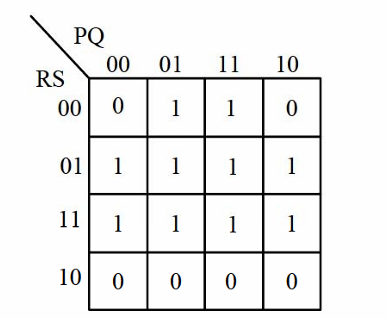
\includegraphics[width=0.3\columnwidth]{figs/Q 35.png}\caption{}     \label{fig:placeholder}
\end{figure}
\begin{multicols}{4}
\begin{enumerate}
    \item $Q\overline{R} + S$
    \item $Q\overline{R} + \overline{S}$
    \item$QR + S$ 
    \item $QR + \overline{S}$
\end{enumerate}
\end{multicols}
\item In the circuit shown below, X and Y are digital inputs, and Z is a digital output. The equivalent circuit is a\hfill{(GATE EE 2019)}
\begin{figure}[H]
    \centering
    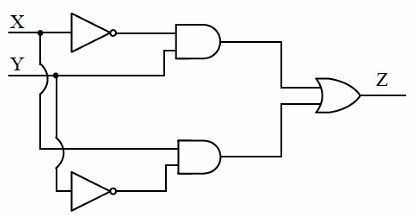
\includegraphics[width=0.4\columnwidth]{figs/Q 36.png}\caption{}     \label{fig:placeholder}
\end{figure}
\begin{multicols}{4}
\begin{enumerate}
    \item NAND gate
    \item NOR gate
    \item XOR gate 
    \item XNOR gate
\end{enumerate}
\end{multicols}

\item A DC-DC buck converter operates in continuous conduction mode. It has 48~V input voltage, and it feeds a resistive load of 24~$\Omega$. The switching frequency of the converter is 250~Hz. If switch-on duration is 1~ms, the load power is\hfill{(GATE EE 2019)}

\begin{multicols}{4}
\begin{enumerate}
    \item 6W
    \item 12W
    \item 24W 
    \item 48W
\end{enumerate}
\end{multicols}

\item The line currents of a three-phase four wire system are square waves with amplitude of 100~A. These three currents are phase shifted by 120$^\circ$ with respect to each other. The rms value of neutral current is\hfill{(GATE EE 2019)}
\begin{multicols}{4}
\begin{enumerate}
    \item 0~A
    \item $\dfrac{100}{\sqrt{3}}$~A
    \item 100~A 
    \item 300~A
\end{enumerate}
\end{multicols}

\item If $\vec{A} = 2x\hat{i} + 3y\hat{j} + 4z\hat{k}$ and $u = x^{2} + y^{2} + z^{2}$, then $\mathrm{div}(u\vec{A})$ at (1, 1, 1) is \underline{\hspace{2cm}}.\hfill{(GATE EE 2019)}

\item The probability of a resistor being defective is 0.02. There are 50 such resistors in a circuit. The probability of two or more defective resistors in the circuit (round off to two decimal places) is \underline{\hspace{3cm}}.\hfill{(GATE EE 2019)}
\vfill
\noindent\rule{\linewidth}{0.4pt}
EE \hfill 8/13
\newpage
\raggedright{GATE 2019 Electrical Engineering (Set No)}
\noindent\rule{\linewidth}{0.4pt}

\item A 0.1  $\mu$ F capacitor charged to 100 \, V is discharged through a 1 k$\Omega$ resistor. The time in ms (round off to two decimal places) required for the voltage across the capacitor to drop to 1 V is \underline{\hspace{2cm}}.\hfill{(GATE EE 2019)}

\item The current $I$ flowing in the circuit shown below in amperes is \underline{\hspace{2cm}}.\hfill{(GATE EE 2019)}

\begin{figure}[H]
    \centering
    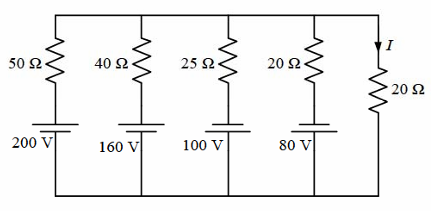
\includegraphics[width=0.5\columnwidth]{figs/Q 42.png}\caption{}     \label{fig:placeholder}
\end{figure}

\item The voltage across and the current through a load are expressed as follows

$v(t) = -170 \sin\left(377 t - \frac{\pi}{6}\right) V$
$i(t) = 8 \cos\left(377 t + \frac{\pi}{6}\right) A$
The average power in watts (round off to one decimal place) consumed by the load is \underline{\hspace{2cm}}.\hfill{(GATE EE 2019)}


\item
The magnetic circuit shown below has uniform cross-sectional area and air gap of 0.2 cm. The mean path length of the core is 40 cm. Assume that leakage and fringing fluxes are negligible. When the core relative permeability is assumed to be infinite, the magnetic flux density computed in the air gap is 1 tesla. With same Ampere-turns, if the core relative permeability is assumed to be 1000 (linear), the flux density in tesla (round off to three decimal places) calculated in the air gap is \underline{\hspace{2cm}}.\hfill{(GATE EE 2019)}

\begin{figure}[H]
    \centering
    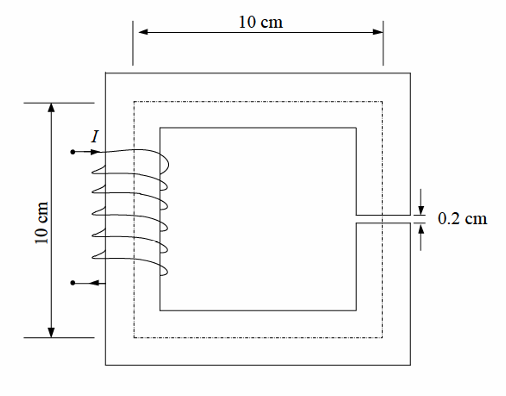
\includegraphics[width=0.6\columnwidth]{figs/Q 44.png}\caption{}     \label{fig:placeholder}
\end{figure}

\item A single-phase transformer of rating 25 kVA, supplies a 12 kW load at power factor of 0.6 lagging. The additional load at unity power factor in kW (round off to two decimal places) that may be added before this transformer exceeds its rated kVA is \underline{\hspace{2cm}}.\hfill{(GATE EE 2019)}

\vfill
\noindent\rule{\linewidth}{0.4pt}
EE \hfill 9/13
\newpage
\raggedright{GATE 2019 Electrical Engineering (Set No)}
\noindent\rule{\linewidth}{0.4pt}

\item A 220 V DC shunt motor takes 3 A at no-load. It draws 25 A when running at full-load at 1500 rpm. The armature and shunt resistances are 0.5~$\Omega$ and 220~$\Omega$, respectively. The no-load speed in rpm (round off to two decimal places) is \underline{\hspace{2cm}}.\hfill{(GATE EE 2019)}
  
  \item A delta-connected, 3.7~kW, 400~V(line), three-phase, 4-pole, 50-Hz squirrel-cage induction motor has the following equivalent circuit parameters per phase referred to the stator: $R_1 = 5.39~\Omega$, $R_2 = 5.72~\Omega$, $X_1 = X_2 = 8.22~\Omega$. Neglect shunt branch in the equivalent circuit. The starting line current in amperes (round off to two decimal places) when it is connected to a 100 V (line), 10 Hz, three-phase AC source is \underline{\hspace{2cm}}.

  \item A 220 V (line), three-phase, Y-connected, synchronous motor has a synchronous impedance of (0.25~+~$j$2.5)~$\Omega$/phase. The motor draws the rated current of 10~A at 0.8~pf leading. The rms value of line-to-line internal voltage in volts (round off to two decimal places) is \underline{\hspace{2cm}}.\hfill{(GATE EE 2019)}

  \item A three-phase 50~Hz, 400~kV transmission line is 300~km long. The line inductance is 1~mH/km per phase, and the capacitance is 0.01~$\mu$F/km per phase. The line is under open circuit condition at the receiving end and energized with 400~kV at the sending end, the receiving end line voltage in kV (round off to two decimal places) will be \underline{\hspace{2cm}}.\hfill{(GATE EE 2019)}

  \item A 30~kV, 50~Hz, 50~MVA generator has the positive, negative, and zero sequence reactances of 0.25~pu, 0.15~pu, and 0.05~pu, respectively. The neutral of the generator is grounded with a reactance so that the fault current for a bolted LG fault and that of a bolted three-phase fault at the generator terminal are equal. The value of grounding reactance in ohms (round off to one decimal place) is \underline{\hspace{2cm}}.\hfill{(GATE EE 2019)}

  \item In the single machine infinite bus system shown below, the generator is delivering the real power of 0.8~pu at 0.8 power factor lagging to the infinite bus. The power angle of the generator in degrees (round off to one decimal place) is \underline{\hspace{2cm}}.\hfill{(GATE EE 2019)}

\begin{figure}[H]
    \centering
    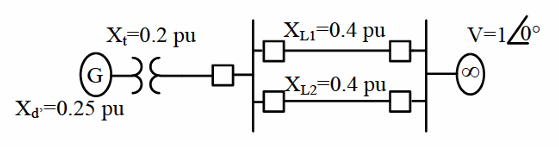
\includegraphics[width=0.7\columnwidth]{figs/Q 51.png}\caption{}     \label{fig:placeholder}
\end{figure}

  \item In a 132~kV system, the series inductance up to the point of circuit breaker location is 50~mH. The shunt capacitance at the circuit breaker terminal is 0.05~$\mu$F. The critical value of resistance in ohms required to be connected across the circuit breaker contacts which will give no transient oscillation is \underline{\hspace{2cm}}.\hfill{(GATE EE 2019)}
\vfill
\noindent\rule{\linewidth}{0.4pt}
EE \hfill 10/13
\newpage
\raggedright{GATE 2019 Electrical Engineering (Set No)}
\noindent\rule{\linewidth}{0.4pt}

\item In a DC-DC boost converter, the duty ratio is controlled to regulate the output voltage at 48~V. The input DC voltage is 24~V. The output power is 120~W. The switching frequency is 50~kHz. Assume ideal components and a very large output filter capacitor. The converter operates at the boundary between continuous and discontinuous conduction modes. The value of the boost inductor (in $\mu$H) is \underline{\hspace{2cm}}.\hfill{(GATE EE 2019)}

    \item A fully-controlled three-phase bridge converter is working from a 415~V, 50~Hz AC supply. It is supplying constant current of 100~A at 400~V to a DC load. Assume large inductive smoothing and neglect overlap. The rms value of the AC line current in amperes (round off to two decimal places) is \underline{\hspace{2cm}}.\hfill{(GATE EE 2019)}

    \item A single-phase fully-controlled thyristor converter is used to obtain an average voltage of 180~V with 10~A constant current to feed a DC load. It is fed from single-phase AC supply of 230~V, 50~Hz. Neglect the source impedance. The power factor (round off to two decimal places) of AC mains is \underline{\hspace{2cm}}.\hfill{(GATE EE 2019)}
    \end{enumerate}
\vfill
\noindent\rule{\linewidth}{0.4pt}
EE \hfill 11/13
\newpage
    \begin{table}[ht]
\centering
\renewcommand{\arraystretch}{2}
\begin{tabular}{|c|c|c|c|c|}
\hline
\textbf{Q.No.} & \textbf{Type} & \textbf{Section} & \textbf{Key} & \textbf{Marks} \\
\hline
1  & MCQ & GA & D & 1 \\
2  & MCQ & GA & C & 1 \\
3  & MCQ & GA & C & 1 \\
4  & MCQ & GA & B & 1 \\
5  & MCQ & GA & D & 1 \\
6  & MCQ & GA & C & 2 \\
7  & MCQ & GA & B & 2 \\
8  & MCQ & GA & A & 2 \\
9  & MCQ & GA & D & 2 \\
10 & MCQ & GA & C & 2 \\
\hline
1  & MCQ & EE & C & 1 \\
2  & MCQ & EE & D & 1 \\
3  & MCQ & EE & B & 1 \\
4  & MCQ & EE & B & 1 \\
5  & MCQ & EE & B & 1 \\
6  & MCQ & EE & A & 1 \\
7  & MCQ & EE & C & 1 \\
8  & MCQ & EE & C & 1 \\
9  & MCQ & EE & C & 1 \\
10 & MCQ & EE & C & 1 \\
11 & MCQ & EE & D & 1 \\
12 & MCQ & EE & B & 1 \\
13 & MCQ & EE & A & 1 \\
\hline
\end{tabular}
\end{table}
\newpage
\begin{table}[ht]
\centering
\renewcommand{\arraystretch}{2}
\begin{tabular}{|c|c|c|l|c|}
\hline
\textbf{Q.No.} & \textbf{Type} & \textbf{Section} & \textbf{Key}         & \textbf{Marks} \\
\hline
14 & MCQ & EE & A                & 1 \\
15 & MCQ & EE & C                & 1 \\
16 & MCQ & EE & B                & 1 \\
17 & MCQ & EE & D                & 1 \\
18 & NAT & EE & 139 to 139       & 1 \\
19 & NAT & EE & 1.3 to 1.5       & 1 \\
20 & NAT & EE & 9 to 11          & 1 \\
21 & NAT & EE & 0.095 to 0.105   & 1 \\
22 & NAT & EE & 100 to 100       & 1 \\
23 & NAT & EE & 100 to 100       & 1 \\
24 & NAT & EE & 3 to 3           & 1 \\
25 & NAT & EE & 111.0 to 115.0   & 1 \\
26 & MCQ & EE & C                & 2 \\
27 & MCQ & EE & A                & 2 \\
28 & MCQ & EE & D                & 2 \\
29 & MCQ & EE & B                & 2 \\
30 & MCQ & EE & B                & 2 \\
31 & MCQ & EE & A                & 2 \\
32 & MCQ & EE & D                & 2 \\
33 & MCQ & EE & C                & 2 \\
34 & MCQ & EE & B                & 2 \\
35 & MCQ & EE & A                & 2 \\
36 & MCQ & EE & C                & 2 \\
\hline
\end{tabular}
\end{table}
\newpage
\begin{table}[ht]
\centering
\renewcommand{\arraystretch}{2}
\begin{tabular}{|c|c|c|l|c|}
\hline
\textbf{Q.No.} & \textbf{Type} & \textbf{Section} & \textbf{Key}         & \textbf{Marks} \\
\hline
37 & MCQ & EE & A OR C              & 2 \\
38 & MCQ & EE & C                   & 2 \\
39 & NAT & EE & 45 to 45            & 2 \\
40 & NAT & EE & 0.25 to 0.27        & 2 \\
41 & NAT & EE & 0.45 to 0.47        & 2 \\
42 & NAT & EE & 0 to 0              & 2 \\
43 & NAT & EE & 585.0 to 590.0      & 2 \\
44 & NAT & EE & 0.820 to 0.850      & 2 \\
45 & NAT & EE & 7.10 to 7.30        & 2 \\
46 & NAT & EE & 1564.00 to 1596.00  & 2 \\
47 & NAT & EE & 13.00 to 16.00      & 2 \\
48 & NAT & EE & 240.00 to 250.00    & 2 \\
49 & NAT & EE & 414.00 to 423.00    & 2 \\
50 & NAT & EE & 1.7 to 1.9          & 2 \\
51 & NAT & EE & 19.0 to 22.0        & 2 \\
52 & NAT & EE & 500 to 500          & 2 \\
53 & NAT & EE & 24 to 24            & 2 \\
54 & NAT & EE & 81.00 to 82.00      & 2 \\
55 & NAT & EE & 0.75 to 0.80        & 2 \\
\hline
\end{tabular}
\end{table}


\end{enumerate}
\end{document}







 \caption{}
    \label{fig:placeholder}



   